\graphicspath{{chapters/inflammation/}}
\chapter{Inflammation}

Biocompatibility is the ability of a material to perform with an appropriate host response in a specific application.
The first system interacting with the scaffold is the immune system, which first gives an immuno response and then starts the healing process. 
Such system can be different tissue by tissue, from healthy or pathologic tissue, etc.
A widespread idea derived from findings in diverse species is that the loss of regenerative capacity is linked to the evolution of immune competence. 
The relationship between tissue healing and the immune response is very complex, since there are both negative and positive roles, depending on the tissue, organ and life stage (embryonic, neonatal or adult). We need to try to reduce inflammation as soon as possible, in order to prioritize healing.
\\
\\
\noindent
If we have a wounded skin in a fetus we will have complete regeneration without scar tissue formation, whereas in adults we observe fibrotic healing. We can take some parameters from the fetal model to try to reduce as much as possible scar tissue formation in adult patients.

\section{Tissue damage}
During the inflammatory response (defence step) we have platelet activation, coagulation, inflammation, leading to bleeding, pathogens, open wound, cell debris. 
Our aim is to block the wound, our body triggers a coagulation cascade. 
Then the system will be activated to regenerate. 
\\
\\
\noindent
In 3-7 days we have migration, proliferation, synthesis, angiogenesis. 
For pathogens we need scar tissue blocking the entrance; inside pathogens need to be addressed by internal inflammation, increase blood flow into the damaged site through angiogenesis (more capillaries).
The overall process in controlled by inflammatory system cells e.g. macrophages. 
Cells are coordinated by interleukines e.g. IL-1, IL-2.
\noindent
What kind of cells are involved? There are three major roles of complement:
\begin{itemize}
\item opsonize particles for phagocytosis (need only reach the C3b stage). Phages can recognize the mark through integrins.
\item elicit inflammatory reaction by acting on leukocytes, mast cells, endothelium
\item complement-mediated cytolysis
\end{itemize}
\noindent
The processes are described in figure \ref{fig:roles}.

\begin{figure}[ht]
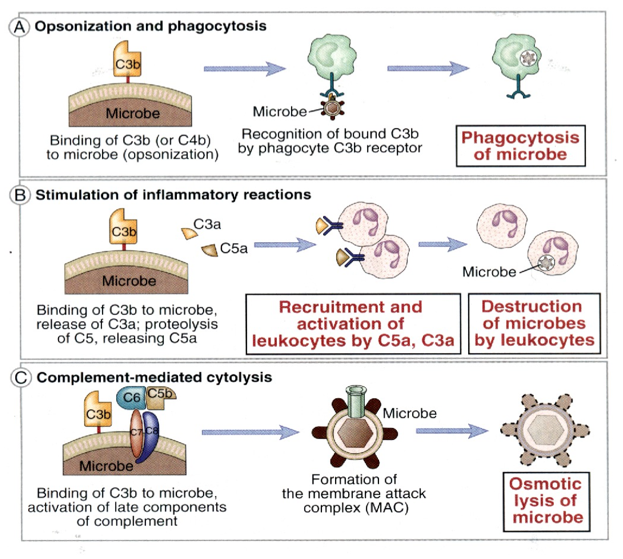
\includegraphics[width=0.6\textwidth]{roles}
\caption{\label{fig:roles}}
\end{figure}

\section{Leukocyte population}

\textbf{Neutrophils/polymorphonuclear} are most abundant circulating leukocytes. 
There are 2 types of intracellular granules, which are common progenitors with monocyte. 
The adult human produces average of $10^11$ per day, with a short life span (6 hours and then apoptosis).
\\
\\
\noindent
\textbf{Monocytes} (and activated macrophages) are phylogenetically the oldest cells of the immune system. 
They circulate as inactive monocytes, enter tissue and become activated macrophages.
They are located in the subepithelial connective tissue, which is present in the interstitia of parenchymal organs, in the lining of vascular sinusoids in liver and spleen and in the lymphatic sinuses of lymph nodes.
Monocytes usually respond later than neutrophils at sites of injury/infection and are the primary effectors of innate immune system.
\\
\\
\noindent
The primary purpose of phagocytes is to clear invading organisms, foreign non-self materials. 
Monocytes can exist for years, while neutrophils live just a few hours.

\section{Phagocyte-mediated wound cleaning}
To produce new vessels from new cells, the mechanism of phagocyte-mediated wound cleaning is the following:
\begin{enumerate}
\item recruitment: adhesion proteins facilitate attachment to endothelium
\item migration: receptors that mediate chemotaxis to target site
\item recognition and phagocytosis: specific receptors for microbes and opsonized materials (phagocytosis) Fc receptors and C3 receptors are major mediators of attachment
\item release of cytotoxic compounds: reactive oxygen and nitrogen species
\item cytokine production secretion of numerous cytokines and chemokines with local and systemic activity:
	 \begin{itemize}
		\item positive factors: increase macrophage activation, recruitment, stimulate adaptive immune system
		\item negative factors: inhibit activation and proliferation
		\item secretion of factors that facilitate wound remodeling, matrix production and angiogenesis
	\end{itemize}
\end{enumerate}
\noindent	
Macrophages dominate biomaterial interfaces in tissue, often present chronically. 
They control the interaction of the scaffold with macrophages and avoid pro inflammatory signals.

\section{Leukocyte extravasation}
Leukocytes travel through blood capillaries. 
Signal molecules (chemotactic signals) first cause leukocytes to adhere to endothelial cells. 
Diffusible chemotactic signals e.g. bacterial peptides result from bacterial degradation in the inflammation site.
The binding of integrins and I-CAM tightens the adhesion and triggers process formation (note this is an exception to the general role of Integrin-ECM interactions).
Additional signals/ligands promote migration.
The overall process is summarized in figure \ref{fig:leuko}.

\begin{figure}[h]
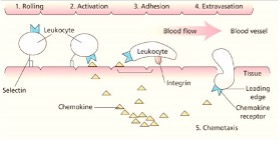
\includegraphics[width=1\textwidth]{leuko}
\caption{\label{fig:leuko}}
\end{figure}
 
\section{TNF alpha}
TNF is the principal mediator of acute inflammation.
Its major source are macrophages and its major effect is the activation of pro-inflammation NFkB transcription factor.
TNF increases the endothelial expression of selectins and integrins, the chemokine production in endothelial cells, macrophage and the production of prostaglandins and leukotrienes (pyrogens, chemotactic). 
Furthermore, it induces prostacyclin expression in endothelium, increases local blood flow and increase IL-1 production in macrophages.

\section{Inflammatory response}
The inflammatory response is the body’s natural response that occurs immediately following tissue damage.
 Its main functions are to defend the body against harmful substances, and to promote the renewal of normal tissue.
Signs of inflammation:
\begin{enumerate}
\item pain: due to chemical released by damaged cells
\item swelling or edema: due to an influx of fluid into the damaged region
\item redness: due to vasodilatation (widening of blood vessels and bleeding in joint or structure)
\item heat: due to an increase in blood flow to the area
\item loss of function: due to increased swelling and pain
\end{enumerate}
\noindent
The inflammatory reaction is the combination of a number of overlapping reactions within the body. 
Although a lot of these occur simultaneously, a certain order of events may be seen.
The tissue damage may occur from trauma such as a tackle, collision or from a fall. 
However, quite commonly tissue injury is as a result of overuse (microtrauma) or pathology
\\
\\
\noindent
When tissue cells become injured, they release a number of chemicals that initiate the inflammatory response. 
Examples of these are kinins, prostaglandin and histamine. 
These chemicals work collectively to cause increased vasodilation (widening of blood capillaries) and permeability of capillaries. 
This leads to increased blood flow to the injured site. 
These substances also act as chemical messengers that attract some of the body’s natural defence cells, in a mechanism that is known as \textbf{chemotaxis}.
Although highly beneficial to the body’s defence strategies, some chemicals also increase the sensitivity of the pain fibres in the area and so the area becomes painful.

\section{Leukocytes migration}
Chemotaxis leads to the migration of certain white blood cells to the damaged area. 
Two types of leukocytes are predominant in the inflammatory response (macrophages and neutrophils). 
Neutrophils are first to reach the injured site and function by neutralising harmful bacteria. Macrophages aid the healing process by engulfing bacteria and dead cells and ingesting them so that the area is clear for new cells to grow. 
They arrive at the injured site within the first 72 hours of the injury and may remain in the area for weeks after the injury.

\section{Wound healing in skin}
We have acute inflammation, proliferation, remodelling and then the reprise of the tensile strength. 
The synthesis of collagen occurs between 7 and 14 days. 
After 14-21 days, we have collagen cross-linking assembling. 
Less cross linking means more flexibility and less strength. 
There is a control of the immune system to induce tissue regeneration.
\\
\\
\noindent
At the beginning we have pro-inflammatory macrophages phagocyte (type I),  which produce cytokines. 
When all the debris has been removed, the macrophages type I become of type II, leading to the downregulation of pro-inflammatory cytokines and tissue regeneration.
Immune tissue engineering is a new approach to drive the transition from type I to type II in order to promote regeneration. 
We need to first release few pro-inflammatory molecules (short response) and then tune the transition.

\noindent
The main actors of the immune response following tissue injury:
\begin{itemize}
\item kinetic of immune cell mobilisation after tissue injury
\item initial inflammatory phase following tissue injury
\item immune mechanisms that can impair tissue healing or drive to scarring and fibrosis
\item pro regenerative immune mechanisms
\end{itemize}

\begin{figure}[h]
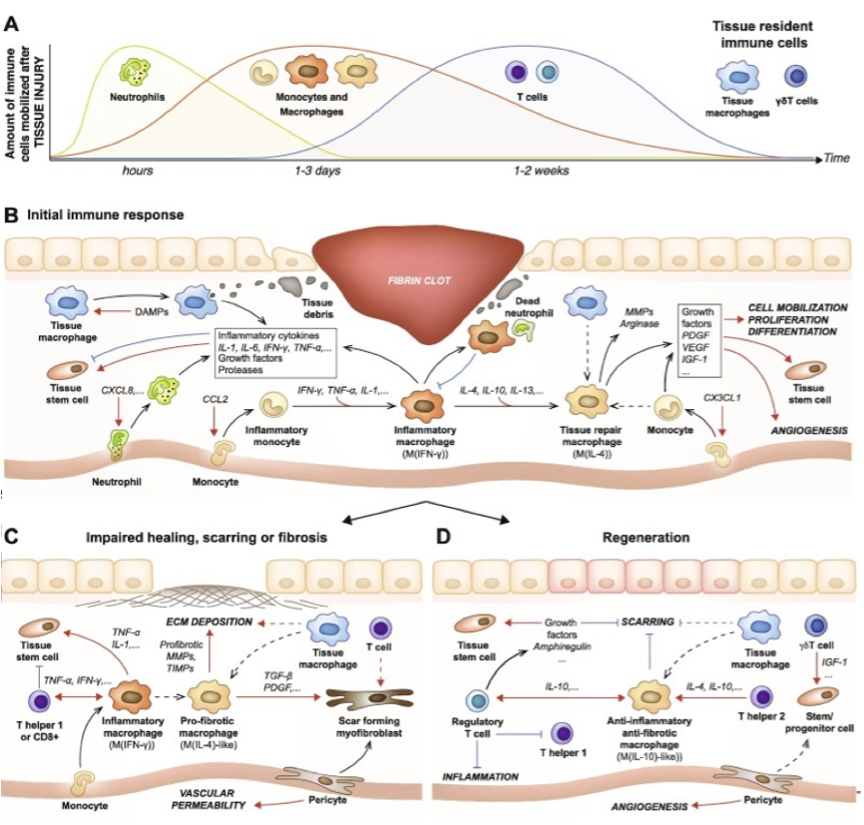
\includegraphics[width=1\textwidth]{healing}
\caption{\label{fig:healing}}
\end{figure}

\section{Strategies to promote tissue regeneration}
Strategies based on biomaterials and drug delivery systems to promote tissue regeneration by controlling the immune system:
\begin{itemize}
\item physicochemical properties of the scaffold. Pay attention to degradability, hydrophobicity, topography…
\item pro-inflammatory modulators
\item anti-inflammatory modulators
\end{itemize}
\noindent
Materials must be chosen according to	protein adsorption, generalised toxic effect, inflammatory cell activation, fibrosis, microvascular changes and tissue-organ specific cell response.

Specific application, tissue-organ type:
\begin{itemize}
\item activation of clotting cascade
\item platelets adhesion activation aggregation
\item complement activation
\item antibody production
\item immune cells response
\item hypersensitivity
\item mutagenesis, genotoxicity
\item tumor formation
\end{itemize}
\noindent
Everything is controlled by the material (type,shape, size, properties) and the environment.
When the biomaterial is recognized as a foreign body, macrophages are recruited and cells will not be able to migrate on the scaffold for regeneration, resulting in a complete failure.

\subsection{Effects of physicochemical modification to biomimetic scaffolds in musculoskeletal applications}
\begin{figure}[h]
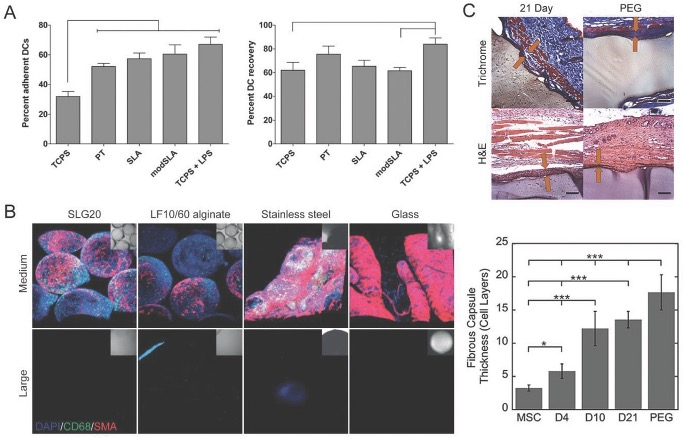
\includegraphics[width=1\textwidth]{muscosk}
\caption{\label{fig:muscosk}}
\end{figure}
In figure \ref{fig:muscosk} we can check the percentage of dendritic cells(inflammatory cells) in the sample. 
We can have a different adhesion degree of inflammatory cells to the scaffold. 
Buffering solution + serum (proteins) + antibiotics + growth factors…depending on the absorption we will have a different cell development. 
In panel B we see the different shape and thickness for each material.
%chiedere altri appunti su questo, poco chiaro

\subsection{Processes affect the biological outcome}
The aim of this experiment is to evaluate the ability an organic membrane to treat skin burn. Absorption is an important property to take into account, because it causes the inflammatory response. 
Keep in mind that proteins can assume different conformations according to specific situation. Three membranes were prepared, they look almost exactly the same. 
By increasing crystallinity the water content is reduced, different mechanical properties (huge rigidity, increased hydrophobicity = less water absorption for the scaffold). 
In vitro tests of the material: fast, easy, not expensive. 
In this case they moved materials A and B into further clinical trials. When moving the material in vivo we will have the incubation with human plasma (reproduce bleeding); the aim is to focus on pro-inflammatory signals.
Chemical production: pro-inflammatory cytokines and mixed environment (pro and anti-inflammatory). Moving down there is increase in opsonin.  Some are stretched, as macrophages lead to more adhesion and activation. 
We observe low adhesion and high inflammation, this is induced by the material for the scaffold. A small amount of proteins is still able to induce a high pro-inflammatory reaction. 

\section{Major activities of macrophages secreted factors}
The main goal of the inflammatory response is healing. 
The system will pass through scar tissue formation, modification and finally regeneration. Macrophages react to inflammation through the killing of microbes (nitric oxide)and phagocytosis. 
%They should find oxotin, produced by the system.  ???
At the beginning we must defense our body from pathogens and next to build up.

\section{Inflammatory monocytes}
\begin{figure}[h]
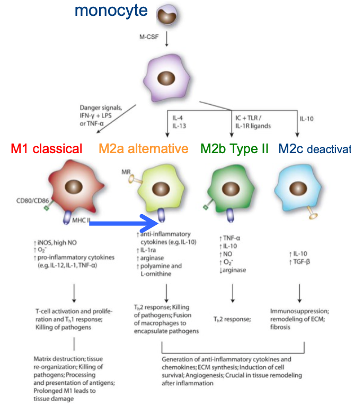
\includegraphics[width=1\textwidth]{mono_diff}
\caption{\label{fig:mono}}
\end{figure}
In figure \ref{fig:mono} we see macrophages differentiation from classical proinflammatory to regenerative. 
Each one is characterized by a specific chemistry. 
Maybe we can employ some of these molecules to witness which kind of macrophage is present. After the interaction between material and inflammatory cell, we must find which will be the inflammatory molecules produced afterwards. 
Sometimes scaffolds are able to produce new ECM, but not new capillaries. 
Our aim is to study when angiogenic factors should be released to induce the regeneration process. 
 
\section{Inflammatory cellular responses}
Opsonin provides the ability for a specific cell to hit the particles and digest them. Phagocytosis involves moving the foreign body from outside to inside within a membrane.
Cancer cells are recognised as foreign since they are coated by opsonin, so they will be eaten by phagocytes.  
Cellular responses: oxidative burst, bacterial killing, tissue injury. 
If the material is very sensitive, it will release pieces, which are destroyed by macrophages and necrotic surrounding tissue. 
The small particles will upregulate the inflammatory response, leading to chronic response. 
Our aim is to reduce as much as possible the intensity and time of the defence, the scar tissue.

\begin{figure}[h]
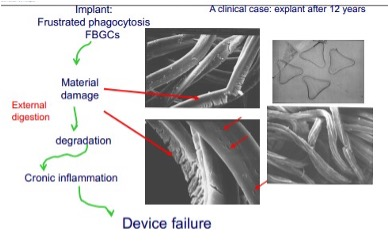
\includegraphics[width=1\textwidth]{failure}
\caption{\label{fig:failure}}
\end{figure}
\noindent
Figure \ref{fig:failure}: interaction between cells and material in an implant, explanted after 12 years due to failure.  
The tube changed its shape and diameter, provoking blood turbulence, thrombosis risk. 
The issue is that spaces were occupied by macrophages, which were able to adhere and digest the external fibers - released in microparticles. 
The protasis was made in nylon, which is considered to be the most stable polymer e.g. used for parachutes. 
Since it is stable and strong, the human body sensed it as foreign and started damaging it. T
he section of the damaged fibers was triangular, while circular fibers had no impact whatsoever. 
What does it mean to try to digest a foreign body? The phagocytes digest it piece by piece and this leads to chronic inflammation and failure.

\section{Tissue Healing}
\begin{enumerate}
\item collagenation and cartilarisation
\item angiogenesis
\item proliferation
\item remodelling
\end{enumerate}
\noindent
Once sufficient cleansing of the area has been achieved, the damaged area begins to sprout new capillaries to bring blood to the region - this is known as angiogenesis or revascularization. 
When blood flow has been re-introduced to the area specific tissue cells begin to re-grow for example in a muscle tear muscle cells with repopulate the area. 
Wound healing occurs towards the end of the inflammatory process, however the two processes overlap considerably. 
\\
\\
\noindent
Macrophages work to clear the damaged area and make space for the regeneration of the new tissue. 
After a number of days, fibroblasts (collagen producing cells) begin to construct a new collagen matrix which will act as the framework for new tissue cells.
Tissue healing occurs with the sprout of new capillaries to bring blood to the region (revascularization). 
Cellular responses in tissue repair: the capillary should not go randomly, the scaffold architecture should also consider space for angiogenesis.
 We must also ensure a path for interconnection by playing with architecture and release of angiogenetic factors.
\\
\\
\noindent
The proliferation phaset lasts 4 weeks. 
In cases where the injury has been more severe, the affected area may be composed by a mixture between specific tissue cells (such as muscle cells) and other tissue known as granulation tissue. 
If this granulation tissue is not removed it will remain and form scar tissue, which can lead to a decreased functional ability of the tissue.
\\
\\
\noindent
The remodelling occurs when the new cells mould into their surrounding to once again produce a functional tissue. 
This process of remodelling can take months even years, altering the new tissue slowly. 
The new cells and protein fibers become arranged in a way that is best suited to the stresses imposed on the tissue. 
Hence, when a tissue is healing ,it is important to stretch it in the correct direction so to optimise the strength of the new tissue.

\section{Rethinking regeneration: empowerment of stem cell by inflammation}
Immune cells at the site of tissue injury, including macrophages and T cells, secrete TNFalpha, TNFy, IL-1, IL-13 and other pro-inflammatory cytokines, which in turn can activate stem cells. 
Once licensed by these cytokines, stem cells can facilitate tissue regeneration though cell differentiation and the release of anti-inflammatory cytokines and growth factors.

\section{Designing immuno informed biomaterials matrices}
We need to provide safety paying attention to tumorigenesis.
There is also the use of extracellular vesicles to load drugs.
We can play with the surface topography or chemistry to design the matrix.
Another aspect that we need to take into account is the macrophage polarization and network formation.
The network should be formed in 3D on the surface, interconnections for macrophages.
For instance, if we have an implanted scaffold we first observe protein adsorption. 
After this we have adhesion, macrophages can adhere by forming a network speeding up the process towards regeneration. 
Macrophages are also involved in vascularization. 
When the scaffold is not porous the macrophages will not be able to polarize and switch to state II, they induce the formation of scar tissue.

\section{Effect of topography and stiffness on macrophages polarisation}
Macrophages assume an elongated shape, M2 like phenotype (up-regulated expression of arginase), on PDMS substrates with 2 gratings topography compared to planar control.
After the adhesion (f), cells start to polarize (g) [figure\ref{fig:topo}] .  Increased stiffness in hydrogel drives the transition in absence of cytokines stimulation. 

\begin{figure}[h]
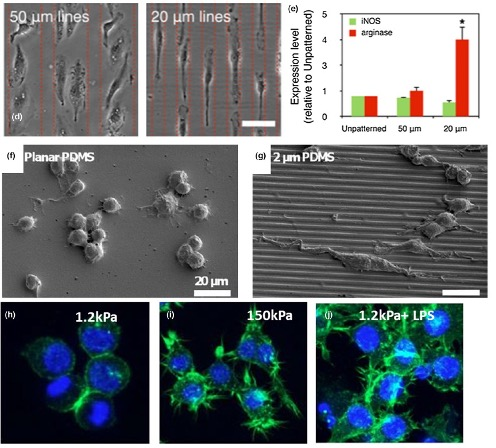
\includegraphics[width=1\textwidth]{topo}
\caption{\label{fig:topo}}
\end{figure}

\section{Role of pore size/distribution/degradation}
\begin{figure}[h]
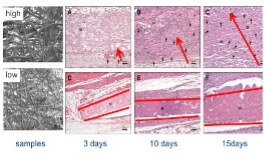
\includegraphics[width=1\textwidth]{silk}
\caption{\label{fig:silk}}
\end{figure}

Figure \ref{fig:silk}: silk fibroin micro-nets formic acid treated (in vivo evaluations). 
In this case we have induced regeneration in unnatural conditions. 
Changing the pore size, the mechanical properties will be affected. In high porosity samples: after 3 days we have granulated tissue (dots are cells), the scaffold was able to promote movement inside. 
At 10 days the arrows are indicating new capillaries. 
Macrophages are at phase II, cells have more space to build tissue. 
Then thinner fibers, blood vessels, not so many dots, signalling that inflammatory cells almost disappeared. 
Already after 3 days we have a very clear scar tissue formation, which becomes thinner in 10 days. 

We have also different vascularisation and degradation that depend on porosity.
